\section{Proposed Method}
\label{sec:method}

\subsection{Preliminaries}

Let $\mathcal{G} = (\mathcal{V}, \mathcal{E})$ be an attributed graph with $N = |\mathcal{V}|$ nodes. Each node $i$ has a feature vector $\mathbf{x}_i \in \mathbb{R}^d$ and a binary label $y_i \in \{0, 1\}$ (0 = benign, 1 = fraud). The nodes are partitioned into disjoint training, validation, and test sets. Fraud typically constitutes 3--17\% of nodes, making the problem severely class-imbalanced.

\subsection{Background: GAAP}

GAAP~\cite{duan2025gaap} produces a node representation $\mathbf{h}_i \in \mathbb{R}^D$ for each node $i$ through three stages, then predicts $\hat{\mathbf{y}}_i = \operatorname{softmax}(\mathbf{W} \mathbf{h}_i)$. It is trained with standard cross-entropy:

\begin{equation}
\mathcal{L}_{\text{GAAP}} = -\frac{1}{|\mathcal{T}_{\text{train}}|} \sum_{i \in \mathcal{T}_{\text{train}}} \log \hat{y}_{i, y_i}
\label{eq:gaap}
\end{equation}

\subsubsection{Dynamic Binning Embedding (DyBEM)}

Raw continuous features cannot be fed directly into message passing without fusing distinct semantics. DyBEM addresses this by learning $b$ adaptive bin boundaries per feature dimension. For the $j$-th feature, the bin boundaries $\{q_{j,0}, q_{j,1}, \dots, q_{j,b}\}$ are initialized via decision-tree binning on the training set~\cite{duan2025gaap} and optimized jointly with the GNN. Each scalar value $x_{i,j}$ is then represented as a $b$-dimensional vector where the $m$-th component encodes the fragment-wise membership of $x_{i,j}$ in bin $m$, producing a bin embedding $\mathbf{e}_{i,j} \in \mathbb{R}^{b}$. Features from all $d$ dimensions are stacked to form $\mathbf{E}_i \in \mathbb{R}^{d \times b}$, which is flattened and projected to the GNN's hidden dimension.

\subsubsection{Message-Passing with GraphSAGE}

GAAP employs GraphSAGE~\cite{hamilton2017inductive} with max-pooling aggregation as its GNN backbone. For each node $v$ at layer $l+1$, the update rule is:

\begin{equation}
\mathbf{h}_v^{(l+1)} = \sigma\!\left(\mathbf{W}_{\text{self}}^{(l)} \mathbf{h}_v^{(l)} + \mathbf{W}_{\text{neigh}}^{(l)} \cdot \max_{u \in \mathcal{N}(v)} \sigma_{\text{pool}}\!\big(\mathbf{W}_{\text{pool}}^{(l)} \mathbf{h}_u^{(l)}\big)\right)
\label{eq:sage}
\end{equation}

where $\mathbf{h}_v^{(0)} = \text{MLP}(\mathbf{E}_v)$ is the DyBEM-projected feature, $\mathcal{N}(v)$ denotes the neighborhood of $v$, and $\sigma$ is a ReLU activation. Max-pooling is chosen because it preserves the strongest signals per dimension rather than averaging them away---critical when a fraud node is surrounded by mostly benign neighbors. The output of the final GNN layer is denoted $\mathbf{g}_i \in \mathbb{R}^{d_h}$, representing the node's local \textit{association pattern}.

\subsubsection{Global Pattern Aggregation}

To mitigate over-smoothing and capture long-range dependencies across the graph, GAAP applies a multi-head cross-attention module. Rather than computing pairwise attention across all $N$ nodes (prohibitively expensive), GAAP caches the GNN output from the previous epoch as historical embeddings $\tilde{\mathbf{G}} \in \mathbb{R}^{N \times d_h}$. For each node $i$, the query is its current GNN output and the keys/values are the cached embeddings:

\begin{equation}
\mathbf{o}_i = \operatorname{MHA}\big(\mathbf{q}_i = \mathbf{g}_i,\; \mathbf{K} = \tilde{\mathbf{G}},\; \mathbf{V} = \tilde{\mathbf{G}}\big)
\label{eq:mha}
\end{equation}

The final representation is a residual combination $\mathbf{h}_i = \alpha \cdot \mathbf{o}_i + (1 - \alpha) \cdot \mathbf{W}_{\text{out}} \mathbf{g}_i$, where $\alpha$ is a learned or fixed mixing coefficient.

\subsection{RP-GAAP: Rare-Pattern Weighted Training}

Under GAAP's equal-weighted loss (Eq.~\ref{eq:gaap}), all training nodes contribute identically to the gradient. Yet the distribution of attribute-association patterns is highly skewed: common patterns dominate, while rare patterns---disproportionately associated with fraud---receive negligible gradient signal. RP-GAAP addresses this by precomputing a rarity weight $w_i$ for each training node.

\paragraph{Pattern construction.}
We select the top-$k$ features by variance over $\mathcal{T}_{\text{train}}$. For each selected feature $j$, we partition its training-set values into $b$ quantile bins with boundaries $q_{j,0} < \cdots < q_{j,b}$. Node $i$ is assigned bin index $c_{i,j}$ where $q_{j, c_{i,j}} \leq x_{i,j} < q_{j, c_{i,j}+1}$. The $k$ bin indices are combined into a single pattern identifier:

\begin{equation}
p_i = \sum_{j \in \mathcal{S}} c_{i,j} \cdot b^{\pi(j)}
\label{eq:pattern}
\end{equation}

where $\mathcal{S}$ is the set of selected feature indices and $\pi(j)$ maps each feature to its position in the set.

\paragraph{Weight assignment.}
Let $f(p) = |\{i \in \mathcal{T}_{\text{train}} : p_i = p\}|$ be the frequency of pattern $p$ in the training set. We linearly interpolate between 1.0 (most frequent) and $w_{\text{max}}$ (rarest), then apply a multiplicative boost $\phi \geq 1$ to fraud nodes, clipped to $[1.0,\; w_{\text{max}} \cdot \phi]$:

\begin{equation}
w_i = \min\!\Big(\!\big[1.0 + (w_{\text{max}} - 1.0) \cdot \frac{\max_q f(q) - f(p_i)}{\max_q f(q) - \min_q f(q)}\big] \cdot \phi^{\mathbb{1}[y_i = 1]},\; w_{\text{max}} \cdot \phi\Big)
\label{eq:weight}
\end{equation}

Nodes not in $\mathcal{T}_{\text{train}}$ receive $w_i = 1.0$. The weight vector $\mathbf{w} \in \mathbb{R}^N$ is computed once before training on CPU (adding $<$1~second overhead) and requires no gradients.

\paragraph{RP-GAAP loss.}
We replace the uniform average in Eq.~\ref{eq:gaap} with a weighted sum:

\begin{equation}
\mathcal{L}_{\text{RP-GAAP}} = -\frac{1}{\sum_{i \in \mathcal{T}_{\text{train}}} w_i} \sum_{i \in \mathcal{T}_{\text{train}}} w_i \cdot \log \hat{y}_{i, y_i}
\label{eq:rpgaap}
\end{equation}

The GAAP forward pass (DyBEM $\to$ GraphSAGE $\to$ MHA $\to$ classifier) is entirely unchanged. The method adds exactly 4 hyperparameters---$b$, $k$, $w_{\text{max}}$, $\phi$---and no learned parameters. We use $b=5$, $k=10$, $w_{\text{max}}=3.0$, $\phi=1.5$ across all experiments.

\begin{figure}[htbp]
    \centering
    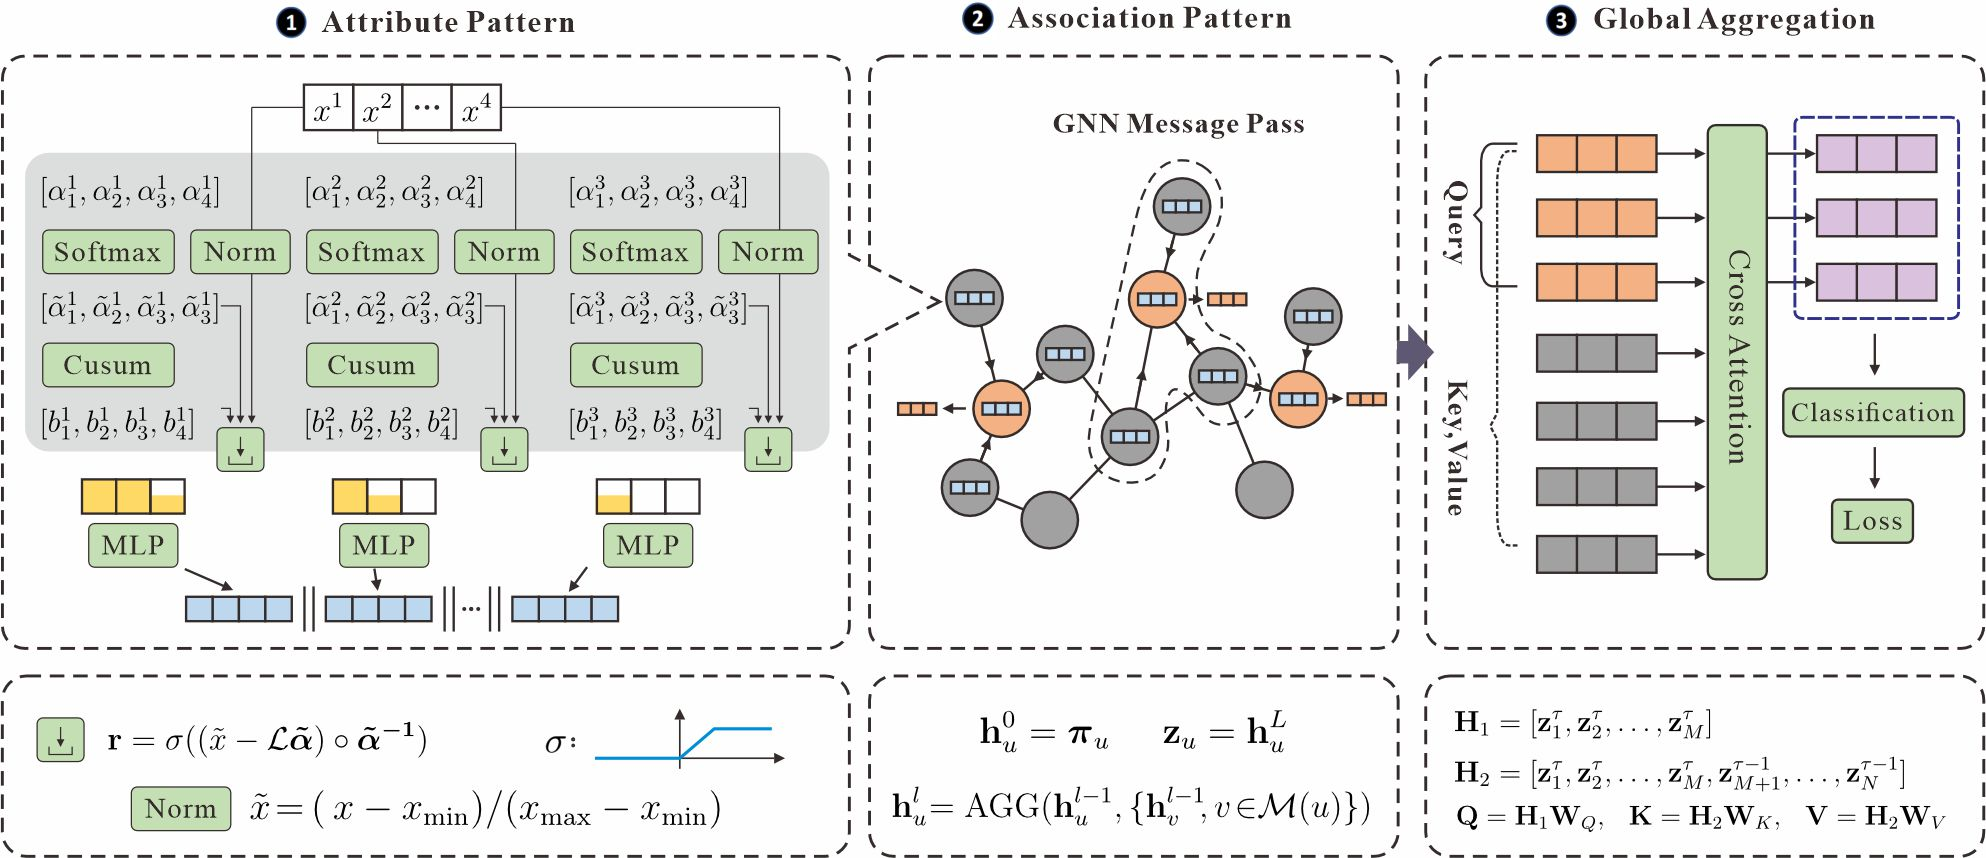
\includegraphics[width=0.95\linewidth]{Figures/framework_crc.jpg}
    \caption{The GAAP framework. DyBEM creates binned attribute patterns, GraphSAGE (Eq.~\ref{eq:sage}) extracts association patterns, and global cross-attention (Eq.~\ref{eq:mha}) captures pattern correlations. RP-GAAP adds rarity weights (Eq.~\ref{eq:weight}) to the loss without modifying this architecture. Figure adapted from Duan et al.~\cite{duan2025gaap}.}
    \label{fig:gaap-framework}
\end{figure}